\chapter{Implementation}
\label{ch:implementation}

This chapter discusses the implementation details and the process of data collection, preprocessing, and algorithms. And we use python to implement our algorithms.

\section{Data Collection}
As mentioned in Section \ref{collection}, COVID-19 related Twitter information should be collected. Twitter provides an official API for a developers to gather data from Twitter. After successfully applying for Twitter developer account, 'consumer key', 'consumer secret', 'access token' and 'access secret' will be generated to be used to connect to Twitter API and access Twitter data. A python library named Tweepy can help the implementation of crawler technology on Twitter. After authentication and biding the key, we can acquire the Twitter information that is needed in this project, and can procure Tweets by searching data, keyword, location, or their combination.

The codes for collecting Twitter data including Tweet, created time, location, username, and ID of Tweet by searching keyword 'COVID-19' are provided in the source code. But still encountered some problems.

\begin{enumerate}
    \item The standard Twitter API only can be used to search Tweets in the last seven days, so there is no way to get earlier data by using it.
    
    \item To manage thousands of request to Twitter API, the number of requests limits are set, and the most common request limit interval is 15 minutes \cite{rate-limits}. The maximum number of requests is 150 times every 15 minutes, which means if the API was repeatedly called beyond the limit, the program would sleep for a while. It significantly reduces the efficiency of data collection. During the implementation, because of the limit, the program ran for over an hour even can only get the Tweets of 20 minutes (for example, get the Tweets from 11:40 to 12:00).
    
    \item When searching data by date using Tweepy, developers can only set the date instead of the specific time. Therefore, if the program was interrupted, the subsequent data cannot get back by setting the specific time.
    
    \item Due to the international restriction, the domestic connection to Twitter API is unstable. Connection exception would be thrown after connecting for a while and the program would stop. Combined with the second limit, when recalling the program, the previous record cannot be saved and only can get the data from scratch. 
\end{enumerate}

These restrictions cannot be avoided. In order to ensure the smooth progress of the project, an open-sourced dataset was found to suit this project. The dataset can be accessed in  \href{https://github.com/echen102/COVID-19-TweetIDs}{Github}. This dataset was collected by keywords tracking and the following figure \ref{fig:4} is a sample of the keywords list \cite{chen2020tracking}.

\begin{figure}[H]
    \centering
    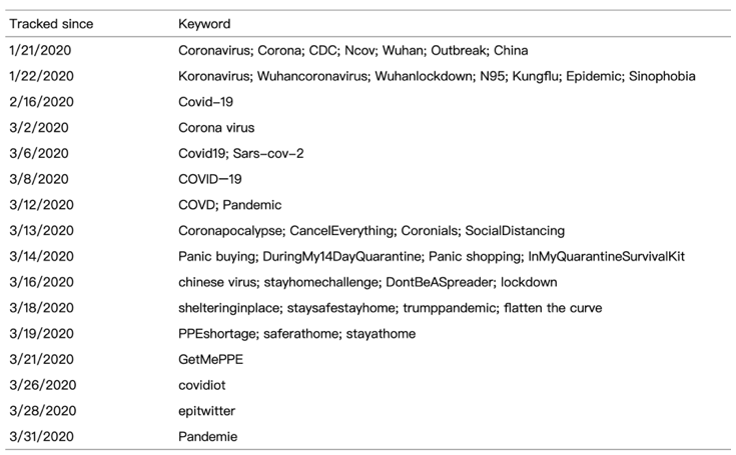
\includegraphics[scale=1.4]{images/keyword.png}
    \caption{Keywords Sample}
    \label{fig:4}
\end{figure}

Additionally, many Twitter datasets only contained the Tweet ID instead of the body text, so we also provided the code to transfer the ID to the text in Twitter.

\section{Preprocessing}
Since there are many defects for raw data to be analyzed such as inconsistencies, noise and missing values \cite{ramirez2017survey}, data preprocessing is a pivotal stage in text clustering framework, and the same as feature extraction and feature selection, preprocessing also has a substantial impact on the effectiveness of cluster model \cite{uysal2014impact}. According to the extensive research \cite{uysal2014impact}, the accuracy of classification or cluster can be improved by choosing suitable preprocessing tasks. Some preprocessing techniques refer to \cite{10.1007/978-3-319-67008-9_31}

\subsection{Structure Unification}
To unify the metadata, for each Tweet, three keys 'Time', 'Location' and 'Text' are set. The unified form for Time is 'yyyy-MM-dd', and for those Tweets without location information, the location key will be set to Null.

\subsection{Data Regularization}
As illustrated in Section \ref{preprocessing}, to get the pure text for the subsequent clustering, regularization should be used on the original Tweets. There is no common regularization rule on all text preprocessing to suit all tasks since the variety of the structure for text data. Based on observation of our Twitter data, the followings are the primary regularization techniques we use for preprocessing the Tweets:

\begin{enumerate}
    \item Remove URL: some tweets might contain URL started with “http” or “www” which would not be needed in the later clustering and should remove them. The regular expression of URLs is “(www$\backslash$.[\^{}$\backslash$s]+)$|$(https?://[\^{}$\backslash$s]+)”.
    
    \item Remove @user: people would like to mention other users in tweets by @ which have no contribution to the analysis and should be removed. The regular expression of it is “@[\^{}$\backslash$s]+”.
    
    \item Remove \#: in front of the hashtag, there is a pound sign which should be removed. And its regular expression is “\#([\^{}$\backslash$s]+)”.
    
    \item Remove multiple marks: some users prefer using multiple marks to express their feelings and would not have meanings for our project. For example, the regular expression for multiple exclamation marks is “($\backslash$!)$\backslash$1+”, and other marks have a similar expression.
    
    \item Remove emoticons: the emoticons have no contribution for NLP. The regular expression example for them is “$:-D|=D|:P$”.
    
    \item Remove emojis: there is a library named \href{https://pypi.org/project/emoji/}{emoji (version 0.6.0)} in Python can import the whole emoji list and can replace emojis into regular text by a function call. Then the emojis can be removed by using the regularization of the replaced text.
    
\end{enumerate}

\subsection{Further Preprocessing Techniques}

To implement the designed preprocessing requirements, an NLP package in python named \href{http://www.nltk.org/install.html}{NLTK)} can be installed. The techniques in NLTK that we can use including removing stopwords, stemming, removing all punctuation, lowercase all characters, and tokenization, which are all mentioned in section \ref{preprocessing}. Additionally, to replace slang words and abbreviations with their equivalent, a file named slang.txt which contains the common slang words and their corresponding written words is imported in our project to help to check the slang.

\section{Algorithm Implementation}
As designed in section \ref{model_design}, in this project, we will implement several algorithms including both word-embedding-based clustering algorithms and probabilistic-based clustering algorithm from feature extraction technique TF-IDF combined with basic clustering model K-means, to advanced topic model BTM. 

Both K-means and LDA can be implemented by python libraries. Library sklearn provides APIs that can help us to achieve TF-IDF and K-means. Load the train texts and prepared the basic requirement such as dictionary and corpus, then K-means text clustering algorithm can be implemented. Library Genism, an open-sourced python package, can be used to implement unsupervised learning of the latent topic expression from unstructured raw text data, which provides the algorithm of LDA topic model. After setting the parameters (the number of topic $K$) and preparing the corpus and dictionary, LDA can be trained.

Though the above two algorithms are simple to implement, at the middle stage of the project, based on some research and experiments, LDA did not perform well on short text data like our Twitter dataset, thus we should begin to attempt another probabilistic based clustering algorithm BTM. 

\begin{algorithm}[H]
  \SetAlgoLined
  \KwIn{documents set $D={d_1,..,d_n}$, topic number $K$, $\alpha$ and $\beta$}
  \KwOut{the topic-word distribution $\vec\theta$ and $\vec\varphi$}
  Preprocess each documents in $D$, build the vocabulary set and encode the documents with the indexes of words\;
  Initialize biterm set $B={}$
  \ForEach{document $d\in D$}{
    Generate all biterms $b_d$ in $d$\;
    Append biterms $b_d$ to biterm set $B$
  }
  Randomly assign a topic $z$ to all biterms in $B$\;
  \For{$iter=1$ to $N_{iter}$}{
    \ForEach{biterm $b_i\in B$}{
        Compute and update $\theta_z=\frac{n_z+\alpha}{|B|+K\alpha}$\;
        \ForEach{$w\in b_i$}{
            Compute and update $\varphi_{w|z}=\frac{n_{w|z}+\beta}{\sum_{w}n_{w|z}+W\beta}$\;
        }
        Compute $P(z|B)=\theta_z \cdot \varphi_{w_i|z} \cdot \varphi_{w_j|z}$\;
        Re-assign topic $z$ to biterm $b_i$\;
        Update $n_z$, $n_{w_i|z}$ and $n_{w_j|z}$\;
    }
    Obtain the final $\vec\theta$ and $\vec\varphi$\;
  }
  \caption{Implementation of BTM Training}
\end{algorithm}

And the algorithm for TTM is very similar to BTM:

\begin{algorithm}[H]
  \SetAlgoLined
  \KwIn{documents set $D={d_1,..,d_n}$, topic number $K$, $\alpha$ and $\beta$}
  \KwOut{the doc-topic distribution $\vec\theta$ and topic-word distribution $\vec\varphi$}
  Preprocess each documents in $D$, build the vocabulary set and encode the documents with the indexes of words\;
  Initialize triterm set $T={}$
  \ForEach{document $d\in D$}{
    Generate all biterms $b_d$ in $d$\;
    Append triterms $b_d$ to biterm set $T$
  }
  Randomly assign a topic $z$ to all triterms in $T$\;
  \For{$iter=1$ to $N_{iter}$}{
    \ForEach{triterm $t_i\in T$}{
        Compute and update $\theta_z=\frac{n_z+\alpha}{|T|+K\alpha}$\;
        \ForEach{$w\in t_i$}{
            Compute and update $\varphi_{w|z}=\frac{n_{w|z}+\beta}{\sum_{w}n_{w|z}+W\beta}$\;
        }
        Compute $P(z|T)=\theta_z \cdot \varphi_{w_i|z} \cdot \varphi_{w_j|z} \cdot \varphi_{w_h|z}$\;
        Re-assign topic $z$ to triterm $t_i$\;
        Update $n_z$, $n_{w_i|z}$, $n_{w_j|z}$ and $n_{w_h|z}$\;
    }
    Obtain the final $\vec\theta$ and $\vec\varphi$\;
  }
  \caption{Implementation of TTM Training}
\end{algorithm}

With a new document put into the trained TTM, the inference algorithm is as follows:

\begin{algorithm}[H]
  \SetAlgoLined
  \KwIn{a new document $d_{new}$, topic number $K$, $\alpha$ and $\beta$, $\vec\varphi$}
  \KwOut{the topic distribution of the new document $\vec\theta_{new}$}
  Encoding the new documents $d_{new}$\;
  Generate triterm set $T_{new}$ from all triterms in $d_{new}$\;
  Randomly assign a topic $z$ to all triterms in $T_{new}$\;
  \For{$iter=1$ to $N_{iter}$}{
    \ForEach{triterm $t_i\in T$}{
        Compute and update $\theta_z=\frac{n_z+\alpha}{|T|+K\alpha}$\;
        Compute $P(z|T)=\theta_z \cdot \varphi_{w_i|z} \cdot \varphi_{w_j|z} \cdot \varphi_{w_h|z}$\;
        Re-assign topic $z$ to triterm $t_i$\;
        Update $n_z$\;
    }
    Obtain the final $\vec\theta$\;
  }
  \caption{Implementation of TTM Inference}
\end{algorithm}